\documentclass{article}
\usepackage{amsmath}
\usepackage{amssymb}
\usepackage{graphicx}
\title{\textbf{QF605 Project}}
\date{Date: 2019/02/16}
\begin{document}
	\maketitle

\section{Part3 Q1: Present value of CMS product}

\noindent To calculate PV of leg receiving CMS10y semi-annually over the next 5 years, we need to find SABR paramters at different expiries in order to price each CMS rate. To this end, cubic spline interpolation is used between $\alpha$ $\nu$, $\rho$ of $1y$ $\times$ $10y$, $5y\times10y$ and $10y\times10y$ SABR models we have calibrated. Sine there was no expiry lower than 1y for us to interpolate, parameters for 0.5y expiry follows those of 1y expiry. After interpolating all the SABR models, static replication is used to price each CMS rate and PV is the sum of the discounted values of all CMS rates, multiplied by the day count fraction. Here goes the mathematical form:
\begin{align*}
PV_{CMS10y}&=D(0,6m)\times 0.5 \times E^T [S_{6m,10y6m}(6m)] \\&+ D(0,1y) \times 0.5 \times E^T [S_{1y,11y}(1y)]\\&+ \dots 
+D(0,5y) \times 0.5 \times E^T [S_{5y,15y}(5y)]\\&= 0.21360611599647322
\end{align*}

Interpolation profiles are given as follow:\\
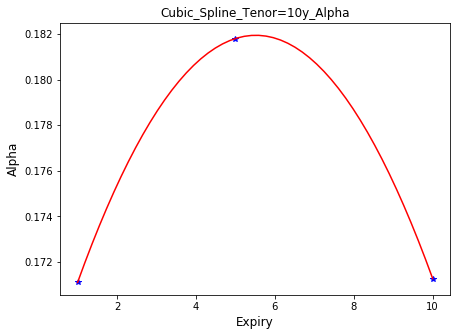
\includegraphics[scale=0.4]{Alpha_10y}\\
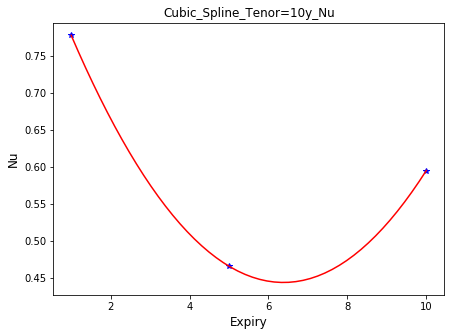
\includegraphics[scale=0.4]{Nu_10y}\\
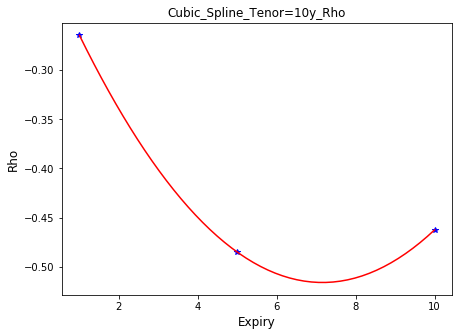
\includegraphics[scale=0.4]{Rho_10y}\\

\noindent Similarly, for CMS2y processed quarterly, $\alpha$ $\nu$, $\rho$ can be interpolated between $1y$ $\times$ $2y$, $5y\times2y$,$10y\times2y$, whose profiles are demonstrated below.\\ In addition to SABR interpolation, due to quarterly arrangement, more discrete OIS discount rates and Libor discount rates are interpolated based on DF calculated in Section 1. After getting all the inputs, we can calculate PV of CMS2y as follow:

\begin{align*}
PV_{CMS2y}&=D(0,3m)\times 0.25 \times E^T [S_{3m,2y3m}(3m)] \\&+ D(0,6m) \times 0.25 \times E^T [S_{6m,2y6m}(6m)]\\&+ \dots 
+D(0,10y) \times 0.25 \times E^T [S_{10y,12y}(10y)]\\&= 0.5048410771318348
\end{align*}

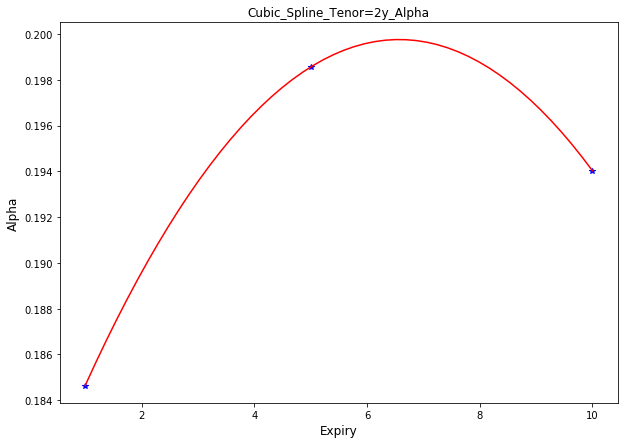
\includegraphics[scale=0.4]{Alpha_2y}\\
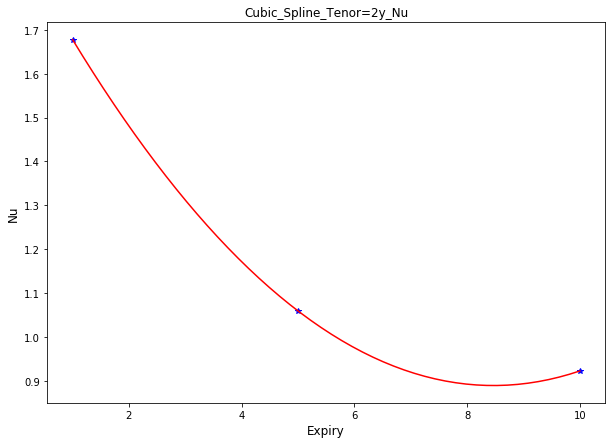
\includegraphics[scale=0.4]{Nu_2y}\\
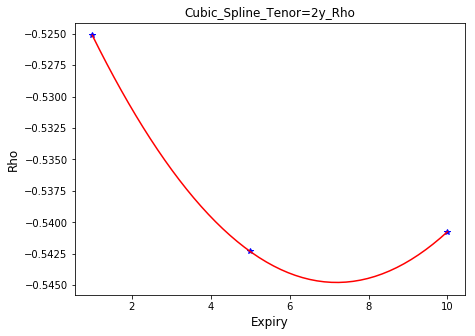
\includegraphics[scale=0.4]{Rho_2y}\\


\end{document}